\begin{figure}[htp]
  \centering
  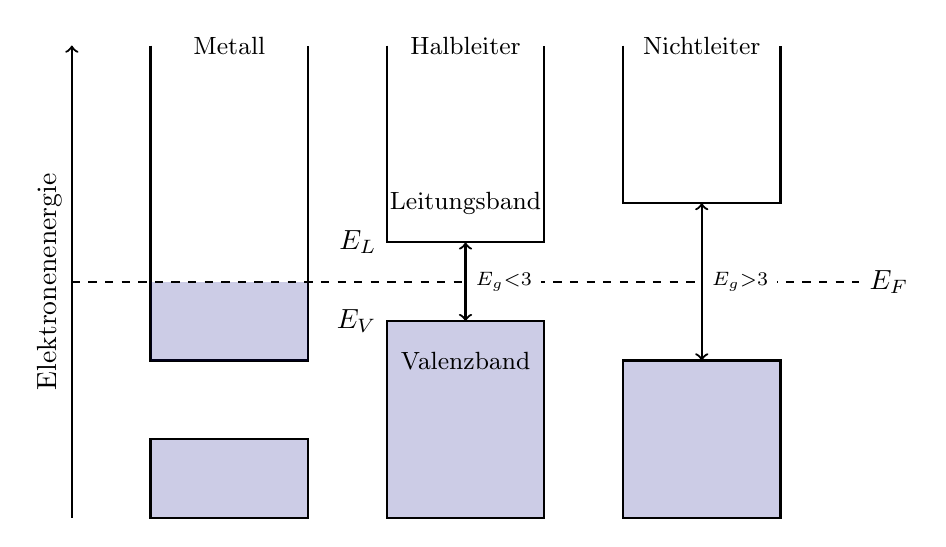
\begin{tikzpicture}
    \draw[thick, ->] (0,0) --node[rotate=90, above]{Elektronenenergie} (0,6);
    \draw[thick] (1,6) -- (1,2) -- (3,2) -- (3,6);
    \fill[fill = blue!50!black, fill opacity = 0.2] (1,2) rectangle (3,3);
    \filldraw[fill = blue!50!black, thick, fill opacity = 0.2] (1,1) rectangle (3,0);
    \node (A) at (2,6){\small Metall};
    \draw[thick] (4,6) -- (4,3.5)node[left]{$E_L$} -- (6,3.5) -- (6,6);
    \filldraw[fill = blue!50!black, thick, fill opacity = 0.2] (4,2.5)node[opacity = 1, left]{$E_V$} rectangle (6,0);
    \node (A) at (5,6){\small Halbleiter};
    \node (A) at (5,2){\small Valenzband};
    \node (A) at (5,4){\small Leitungsband};
    \draw[thick] (7,6) -- (7,4) -- (9,4) -- (9,6);
    \filldraw[fill = blue!50!black, thick, fill opacity = 0.2] (7,2) rectangle (9,0);
    \node (A) at (8,6){\small Nichtleiter};

    \draw[thick, dashed] (0,3) -- (10,3)node[right]{$E_F$};
    \draw[thick, <->] (5,3.5) --node[fill=white, right]{$\scriptstyle E_g < \SI{3}{\electronvolt}$} (5,2.5);
    \draw[thick, <->] (8,4) --node[fill=white, right]{$ \scriptstyle E_g > \SI{3}{\electronvolt}$} (8,2);
  \end{tikzpicture}
  \caption{Bandschema von Metallen, Halbleitern und Nichtleitern. In blau sind die bei $T=\SI{0}{\kelvin}$ besetzten Zustände dargestellt.}
  \label{fig:Bandschema}
\end{figure}
